 %----------------------------------------------------------------------------------------
%   Доорх хэсгийг өөрчлөх шаардлагагүй
%----------------------------------------------------------------------------------------
%!TEX TS-program = xelatex
%!TEX encoding = UTF-8 Unicode
\documentclass[12pt,A4]{report}

\usepackage{fontspec,xltxtra,xunicode}
\setmainfont[Ligatures=TeX]{Times New Roman}
\setsansfont{Arial}

% \usepackage[utf8x]{inputenc}
% \usepackage[mongolian]{babel}
%\usepackage{natbib}
\usepackage{geometry}
%\usepackage{fancyheadings} fancyheadings is obsolete: replaced by fancyhdr. JL
\usepackage{fancyhdr}
\usepackage{float}
\usepackage{afterpage}
\usepackage{graphicx}
\usepackage{amsmath,amssymb,amsbsy}
\usepackage{dcolumn,array}
\usepackage{tocloft}
\usepackage{dics}
\usepackage{nomencl}
\usepackage{upgreek}
\newcommand{\argmin}{\arg\!\min}
\usepackage{mathtools}
\usepackage[hidelinks]{hyperref}

\usepackage{algorithm}
\usepackage{algpseudocode}

\usepackage{listings}
\DeclarePairedDelimiter\abs{\lvert}{\rvert}%
\makeatletter
\usepackage{caption}
\captionsetup[table]{belowskip=0.5pt}
\usepackage{subfiles}

\usepackage{listings}
\renewcommand{\lstlistingname}{Код}
\renewcommand{\lstlistlistingname}{\lstlistingname ын жагсаалт}

\usepackage{color}
\definecolor{codegreen}{rgb}{0,0.6,0}
\definecolor{codegray}{rgb}{0.5,0.5,0.5}
\definecolor{codepurple}{rgb}{0.58,0,0.82}
\definecolor{backcolour}{rgb}{0.99,0.99,0.99}
 
\lstdefinestyle{mystyle}{
    basicstyle=\ttfamily\small,
    backgroundcolor=\color{backcolour},   
    commentstyle=\color{codegreen},
    keywordstyle=\color{magenta},
    numberstyle=\tiny\color{codegray},
    stringstyle=\color{codepurple},
    %basicstyle=\footnotesize,
    breakatwhitespace=false,         
    breaklines=true,                 
    captionpos=b,                    
    keepspaces=false,                 
    numbers=left,                    
    numbersep=10pt,                  
    showspaces=false,                
    showstringspaces=true,
    showtabs=false,                  
    tabsize=2
}
 
\lstset{style=mystyle, label=DescriptiveLabel} 

\let\oldabs\abs
\def\abs{\@ifstar{\oldabs}{\oldabs*}}
\makenomenclature
\begin{document}


%----------------------------------------------------------------------------------------
%   Өөрийн мэдээллээ оруулах хэсэг
%----------------------------------------------------------------------------------------

% Дипломийн ажлын сэдэв
\title{DDPG бататгасан сургалтын үйлдлийн шуугианыг турших, харьцуулах }
% Дипломын ажлын англи нэр
\titleEng{Effect of action space noise for DDPG RL algorithm}
% Өөрийн овог нэрийг бүтнээр нь бичнэ
\author{Батбаярын Бямбаням}
% Өөрийн овгийн эхний үсэг нэрээ бичнэ
\authorShort{Б.Бямбаням}
% Удирдагчийн зэрэг цол овгийн эхний үсэг нэр
\supervisor{Г.Гантулга}
% Хамтарсан удирдагчийн зэрэг цол овгийн эхний үсэг нэр
\cosupervisor{}

% СиСи дугаар 
\sisiId{17B1NUM1479}
% Их сургуулийн нэр
\university{МОНГОЛ УЛСЫН ИХ СУРГУУЛЬ}
% Бүрэлдэхүүн сургуулийн нэр
\faculty{ХЭРЭГЛЭЭНИЙ ШИНЖЛЭХ УХААН, ИНЖЕНЕРЧЛЭЛИЙН СУРГУУЛЬ}
% Тэнхимийн нэр
\department{МЭДЭЭЛЭЛ, КОМПЬЮТЕРИЙН УХААНЫ ТЭНХИМ}
% Зэргийн нэр
\degreeName{Бакалаврын судалгааны ажил}
% Суралцаж буй хөтөлбөрийн нэр
\programeName{Мэдээллийн технологи (D061304)}
% Хэвлэгдсэн газар
\cityName{Улаанбаатар}
% Хэвлэгдсэн огноо
\gradyear{2021 оны 02 сар}


%----------------------------------------------------------------------------------------
%   Доорх хэсгийг өөрчлөх шаардлагагүй
%----------------------------------------------------------------------------------------
%----------------------Нүүр хуудастай хамаатай зүйлс----------------------------
\pagenumbering{roman}
\makefrontpage
\maketitle

\doublespace

% Decleration
\begin{huge}
\textbf{Зохиогчийн баталгаа}
\end{huge} \\ \ \\ 
\doublespace
Миний бие \@author \ "\@title" \ сэдэвтэй судалгааны ажлыг гүйцэтгэсэн болохыг зарлаж дараах зүйлсийг баталж байна:
\begin{itemize}
\item Ажил нь бүхэлдээ эсвэл ихэнхдээ Монгол Улсын Их Сургуулийн зэрэг горилохоор дэвшүүлсэн болно.
\item Энэ ажлын аль нэг хэсгийг эсвэл бүхлээр нь ямар нэг их, дээд сургуулийн зэрэг горилохоор оруулж байгаагүй.
\item Бусдын хийсэн ажлаас хуулбарлаагүй, ашигласан бол ишлэл, зүүлт хийсэн.
\item Ажлыг би өөрөө (хамтарч) хийсэн ба миний хийсэн ажил, үзүүлсэн дэмжлэгийг дипломын ажилд тодорхой тусгасан. 
\item Ажилд тусалсан бүх эх сурвалжид талархаж байна. 
\end{itemize} 
\ 

Гарын үсэг: \underline{\hspace{5cm}} 

Огноо: 	\ \ \underline{\hspace{3cm}}

% Гарчгийг автоматаар оруулна
\setcounter{tocdepth}{1}
\tableofcontents

% Зургийн жагсаалтыг автоматаар оруулна
\listoffigures

% Хүснэгтийн жагсаалтыг автоматаар оруулна
\listoftables

% Кодын жагсаалтыг автоматаар оруулна
\lstlistoflistings

% This puts the word "Page" right justified above everything else.
\newpage
%% \addtocontents{lof}{Зураг~\hfill Хуудас \par}
\newpage
%% \addtocontents{lot}{Хүснэгт~\hfill Хуудас \par}

\renewcommand{\cftlabel}{Зураг}

\begin{huge}
\textbf{Товчилсон үг}
\end{huge}
\doublespace

DDPG - Deep Deterministic Policy Gradient

RL - Reinforcement learning

DNN - Deep Neural Network

ANN - Artificial Neural Network

LR - Learning rate

\doublespace
\pagenumbering{arabic}


% Удиртгалыг оруулж ирэх ба abstract.tex файлд удиртгалаа бичнэ
\begin{abstract}
  Reinforcement learning буюу бататгасан сургалтад тасралттай үйлдлийн хувьд суралцах үйл явц нь санамсаргүй үйлдлийг сонгох замаар явагддаг. Харин үргэлжилсэн үйлдлийн хувьд суралцах үйл явц нь үйлдэлд шуугианыг нэмэх замаар явагддаг. Deep Deterministic Policy Gradient (DDPG) бол тасралтгүй, үргэлжилсэн үйлдлүүдийг сурахад зориулагдсан алгоритм тул action space noise буюу үйлдлийн шуугиан ашиглагдана. Энэ судалгааны ажлаар 3 төрлийн шуугианыг харьцуулах, турших бөгөөд ямар үр нөлөөтэй, аль шуугиан нь илүү болохыг тодорхойлно.
  
\section{Зорилго}

DDPG бататгасан сургалтын үйлдлийн шуугианыг туршин, харьцуулж энэ шуугиан моделийг сургах үйл явцад хэрхэн нөлөөлж буйг ажиглан дүгнэлт гаргах

\section{Зорилтууд}

\begin{itemize}
	\item Моделийг DDPG алгоритмыг ашиглан BiPedalWalker-V3 орчныг дуустал алхаж чаддаг болгох
	\item Бие биенээсээ хамааралтай шуугиан, бие биенээсээ хамааралгүй шуугиан, параметр шуугиан гэх гурван төрлийн шуугианыг амжилттай хэрэгжүүлэх
	\item Хэрэгжүүлэлт хийхдээ кодыг аль болох ойлгомжтой DDPG алгоритын pseudo кодын дагуу хэрэгжүүлэх
\end{itemize}
  
\end{abstract}


%----------------------------------------------------------------------------------------
%   Дипломын үндсэн хэсэг эндээс эхэлнэ
%----------------------------------------------------------------------------------------
%\addcontentsline{toc}{part}{БҮЛГҮҮД}
% Шинэ бүлэг

\chapter{Судалгаа}

Энэ хэсэгт RL-ийн цаад санаануудыг болон Deep Deterministic Policy Gradient (DDPG) алгоритмыг ойлгоход шаардлагатай зарим онолыг тайлбарлалаа. Мөн ашигласан технологийн тайлбарыг орууллаа.

\section{Бататгасан сургалтын алгоритм}

DDPG алгоритмыг тайлбарлахаас өмнө Reinforcement Learning буюу бататгасан сургалтын талаар бага зэрэг тайлбарлая. Цаашдаа RL гэж товчлон бичнэ.

RL нь агент болон орчин гэсэн хоёр хэсгээс тогтдог. Орчин гэдэг нь агент ажиллаж байгаа объектыг, агент гэдэг нь RL алгоритмыг илэрхийлнэ.

\begin{figure}[H]
\centering
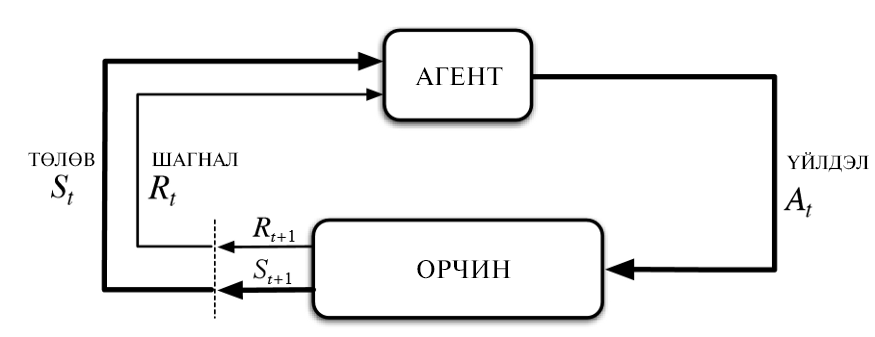
\includegraphics[width=0.8\textwidth]{./images/rl}
\caption{Бататгасан сургалтын бүтэц}
\end{figure}

Орчин нь агентруу төлөвийг илгээх байдлаар эхэлдэг бөгөөд агент нь мэдлэг дээрээ тулгуурлан тухайн нөхцөл байдалд хариу үйлдэл үзүүлнэ. Үүний дараа орчин агент руу дараагийн төлөв болон reward-ыг илгээнэ. Агент нь орчноос хүлээн авсан reward-аар мэдлэгээ шинэчилнэ. Энэ давталт нь орчноос дуусгах төлөв илгээх хүртэл үргэлжилнэ. Ихэнх RL алгоритмууд дээрх байдлаар ажилладаг.

Агентын төлөв байдлыг дүрслэхийн тулд тухайн нөхцөл байдалд агент хэрхэн ажиллах ёстойг тооцоолох полиси (policy) функцийг (агентийн тархи гэсэн үг) тодорхойлдог. Практик дээр полиси (policy) нь ихэвчлэн тоглоомын одоогийн төлөвийг оролт болгон авч зөвшөөрөгдсөн үйлдлүүдийн аль нэгийг хийх магадлалыг тооцдог неорал сүлжээ юм.

Доорх зурагт үзүүлсэн Понг тоглоомд полиси нь дэлгэцийн пикселийг авч тоглогчийн цохиурыг (ногоон) дээш, доош эсвэл хоёуланг нь хөдөлгөх магадлалыг тооцоолж болно. Доорх зурагт полиси нь неорал сүлжээ буюу Hidden layer юм. [6]

\begin{figure}[H]
\centering
\href{https://openai.com/content/images/2017/03/first-graphic-1.png}{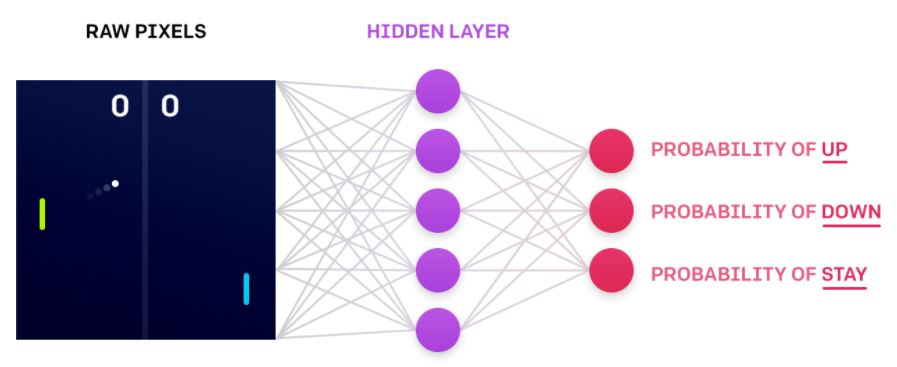
\includegraphics[width=0.8\textwidth]{./images/neural_network}}
\caption{Неороны сүлжээний жишээ}
\end{figure}

\subsection{Бататгасан сургалттай холбоотай нэр томъёо}

\begin{itemize}
	\item Action (A): Агент-ийн хийх боломжтой бүх алхмууд
	\item State (S): Орчноос буцаж ирэх тухайн нөхцөл байдал
	\item Reward (R): өмнөх үйлдлийн үр дүнд гарсан ололт, шагнал
	\item Policy (\(\pi\)): Агент одоогийн төлөв байдалд үндэслэн дараагийн үйлдлийг тодорхойлоход ашигладаг стратеги. 
	\item Value (V): урт хугацааны ололт
	\item Q-value эсвэл action-value(Q): Value-тай төстэй. Гэхдээ одоогийн үйлдлийг нэмэлт параметрээр авдаг.
\end{itemize}

\subsection{Model-free}

Model-free гэдэг нь мэдлэгээ шинэчлэхийн тулд шагналд тулгуурладаг. Төлөвүүд болон үйлдлүүдийг хадгалах шаардлагагүй. 

\subsection{On-policy болон off-policy}

On-policy агент нь value-г одоогийн policy-г ашигласан одоогийн үйлдэлд тулгуурлан сурдаг. Харин off-policy агент өөр нэг policy-г ашигласан үйлдэл a*-д тулгуурлан сурдаг.

\subsection{Суралцах үйл явц}

Reinforcement learning буюу бататгасан сургалтад тасралттай үйлдлийн хувьд суралцах үйл явц нь санамсаргүй үйлдлийг сонгох замаар явагддаг. Харин үргэлжилсэн үйлдлийн хувьд суралцах үйл явц нь үйлдэлд шуугианыг нэмэх замаар явагддаг.

\section{Гүн неороны сүлжээ}

Хиймэл неорал сүлжээ (Artificial Neural Network - ANN) нь тархи хэрхэн ажилладгаас санаа авсан функцийг ойролцоологч (function approximator) юм. ANN нь нэг давхарга дахь неоралууд бүгд урд давхарга дахь неоралуудтай холбогддог хэд хэдэн давхарласан хиймэл неоралаас бүрдэнэ. Бүх хиймэл неоралууд нь идэвхжүүлэх функцтэй байдаг бөгөөд энэ нь ихэвчлэн ReLu функц байдаг. 

\begin{center}
$f(x)=max(0, x)$
\end{center}

$X_j$ нь неоралтай холбогдсон тохиолдолд $w_{ij}$ жинтэй байдаг ба неорал бүр хэвийх утгатай $b_i$ байдаг. Неоралын гаралтыг дараах томъёогоор тооцоолж болно:

\begin{center}
$y=f(b_i+\sum_{h=1}^{n}w_{ij} x_j)$
\end{center}

Эхний давхаргыг оролт болгон ашигласнаар оролтыг өөр давхаргаар дамжуулж, сүлжээний сүүлийн давхаргаас гарах утгыг авах боломжтой. ANN нь илүү нарийн төвөгтэй функцуудийг ойролцоолох боломжтой тохиромжтой олон давхарга, неоралуудтай бол гүн неорал сүлжээ (Deep Neural network - DNN) гэж үздэг. 

\section{DDPG алгоритм}

Deep Deterministic Policy Gradient (DDPG) бол үргэлжилсэн, тасралтгүй үйлдлүүдийг сурахад зориулагдсан model-free off-policy алгоритм юм. Q-функц ба policy-ыг зэрэг сурдаг алгоритм юм. Q-функцийг сурахын тулд off-policy өгөгдөл болон Bellman тэгшитгэлийг ашигладаг. Мөн policy-г сурахын тулд Q-функцыг ашигладаг.  [3]

DDPG алгоритм дараах 4 неорал сүлжээг ашигладаг:
\begin{itemize}
	\item ${\theta}^Q$:Actor сүлжээ
	\item ${\theta}^{\mu}$:Critic сүлжээ
	\item ${\theta}^{Q^{'}}$:target Actor сүлжээ
	\item ${\theta}^{{\mu}^{'}}$:target Critic сүлжээ
\end{itemize} 
 
Actor сүлжээ нь төлөвөөс хамааран үйлдлийг санал болгоно. Төлөвийг оролтоор авч үйлдлийг гаргана. Critic сүлжээ нь төлөвөөс хамаарсан үйлдэл нь сайн эсвэл муу болохын урьдчилан таамагладаг. Төлөв болон үйлдлийг оролтоор авч Q-value-г гаргадаг. Actor сүлжээ нь байнгын суралцаж явдаг бол critic сүлжээ нь аажмаар суралцаж явдаг.

Target network нь суралцсан сүлжээнүүдийг хянаж байдаг эх сүлжээнүүдийнхээ хуулбарууд юм. Эдгээр сүлжээг ашиглан тогтвортой сурах байдлыг сайжруулдаг.	 [2]

Доор DDPG алгоритмын pseudo-code-ыг харууллаа. Үүнийг 4 хэсэгт задлан тайлбарлаж болно. [1]

\begin{itemize}
	\item Туршлагаа хадгалах (Experience replay)
	\item Actor болон critic сүлжээг шинэчлэх
	\item Target сүлжээг шинэчлэх
	\item Судалгаа хийх (Exploration)
\end{itemize} 

\subsubsection{DDPG алгоритмын pseudo code}

$\theta^Q$ болон $\theta^{\mu}$ жинтэйгээр critic сүлжээ $Q(s_i,a_i|\theta^Q)$ болон actor сүлжээ $\mu(s|\theta^mu)$ -г үүсгэнэ

$\theta^{Q{'}} \longleftarrow \theta^Q$, $\theta^{\mu{'}} \longleftarrow \theta^\mu$ жинтэйгээр target сүлжээ $Q^{'}$ болон $\mu^{'}$-г үүсгэнэ

Replay buffer-aa үүсгэнэ

for episode = 1, M do

\quad Анхны төлөв болох s1-г авна

\quad for t = 1, T do

\quad\quad Тухайн policy болон шуугиан дээрээ үндэслэн үйлдлээ сонгоно $a_t = \mu(s_t|\theta^\mu)+N_t$

\quad\quad Үйлдэл $a_t$-гээ гүйцэтгээд reward $r_t$ болон шинэ төлөв $s_t+1$-ээ авна

\quad\quad Replay buffer-даа төлөв, үйлдэл, reward, шинэ төлөвөө ($s_t, a_t, r_t, s_t+1$) хадгалж авна

\quad\quad Replay buffer-аасаа N тооны санамсаргүй утгыг авна

\quad\quad $y_i=r_i+\gamma{Q^{'}}(s_i+1,\mu^{'}(s_i+1|\theta^{\mu^{'}})|\theta^{Q{'}})$ утгыг онооно

\quad\quad Алдааг багасгаж critic сүлжээг шинэчилнэ: $L = \dfrac{1}{N}\sum_{i}(y_i-Q(s_i,a_i|\theta^Q))^2$

\quad\quad Actor policy-г шинэчлэнэ: 
\begin{center}
$\bigtriangledown_\theta\mu J(\theta) \approx \dfrac{1}{N}\sum_{i}[\bigtriangledown_a Q(s, a|\theta^Q)|_s=s_i,a=\mu(s_i)\bigtriangledown_\theta\mu \mu(s|\theta^\mu)|_s=s_i]$
\end{center}

\quad\quad Target сүлжээнүүдийг шинэчлэнэ:
\begin{center}
$\theta^{Q{'}} \longleftarrow \tau\theta^Q + (1-\tau)\theta^{Q{'}}$ 

$\theta^{\mu{'}} \longleftarrow \tau\theta^\mu + (1-\tau)\theta^{\mu{'}}$ 
\end{center}

\quad\quad end for

\quad end for

\subsubsection{Replay buffer}

DDPG алгоритм нь replay buffer-ыг туршлагыг цуглуулахад ашигладаг. Цуглуулсан туршлагаа неороны сүлжээний параметрүүдийг шинэчлэхэд ашигладаг. Value болон policy сүлжээг шинэчлэхдээ replay buffer дахь туршлагуудаас санамсаргүй байдлаар цуглуулан ашигладаг.

Яагаад replay buffer-ыг ашиглаж байгаа вэ гэхээр алгоритмд хамааралгүй байдлаар тархсан өгөгдөл хэрэгтэй. Ийм өгөгдлүүдийг replay buffer дахь туршлагуудаас санамсаргүй байдлаар сонгон авах байдлаар цуглуулж болно.

\subsubsection{Actor болон Critic сүлжээг шинэчлэх}

Critic сүлжээг шинэчлэх үйл явц нь Q-learning-тэй төстэй байдлаар хийгддэг. Шинэчлэгдсэн Q утгыг Беллманы тэгшитгэлээс гарган авна:

\begin{center}
$y_i=r_i+\gamma{Q^{'}}(s_i+1,\mu^{'}(s_i+1|\theta^{\mu^{'}})|\theta^{Q{'}})$
\end{center}

DDPG-д дараагийн төлөв Q утгуудыг target critic network, target actor network ашиглан тооцдог. Дараа нь шинэчлэгдсэн Q утга ба анхны Q утга хоорондын дундаж квадрат алдааг хамгийн бага хэмжээнд хүртэл бууруулна:

\begin{center}
$Loss = \dfrac{1}{N}\sum_{i}(y_i-Q(s_i,a_i|\theta^Q))^2$
\end{center}

Анхны Q утга нь target network-оос биш critic network-оос бодогдон гарна. 

Actor сүлжээний хувьд гол зорилго нь буцан ирэх үр дүн хамгийн дээд хэмжээнд байх юм:

\begin{center}
$J(\theta) = E[Q(s, a)|_{s=s_t,a_t=\mu(s_t)}]$
\end{center}

Actor алдагдлыг тооцоолохын тулд зорилгын функцийн деривативыг авна:

\begin{center}
$\bigtriangledown_\theta\mu J(\theta) \approx \bigtriangledown_a Q(s, a)\bigtriangledown_\theta\mu \mu(s|\theta^\mu)$
\end{center}

Policy-гоо off-policy байдлаар шинэчилж байгаа учир санамсаргүй байдлаар авсан туршлагуудынхаа градиентүүдийн нийлбэрийн дундаж утгыг авна:

\begin{center}
$\bigtriangledown_\theta\mu J(\theta) \approx \dfrac{1}{N} \sum_{i}[\bigtriangledown_a Q(s, a|\theta^Q)|_{s=s_i,a=\mu(s_i)}\bigtriangledown_\theta\mu \mu(s|\theta^\mu)|_{s=s_i}]$
\end{center}

\subsubsection{Target сүлжээг шинэчлэх}
 
Target сүлжээний параметрүүдийг хуулбарлаад, тэдгээрээр дамжуулан сурсан сүлжээнүүдээ хянана. Target сүлжээний параметрүүдийг тодорхой хугацааны алхам хийсний дараа дараах томъёогоор шинэчилдэг:

\begin{center}
$\theta^{Q{'}} \longleftarrow \tau\theta^Q + (1-\tau)\theta^{Q{'}}$ 

$\theta^{\mu{'}} \longleftarrow \tau\theta^\mu + (1-\tau)\theta^{\mu{'}}$ 

$\tau $ бол ихэвчлэн 1-тэй ойролцоо байхаар сонгосон параметр юм (жишээлбэл: 0.999).
\end{center}

\subsubsection{Шуугиан нэмэх}

DDPG алгоритмын баримт бичиг зохиогчид үйлдэлд шуугиан нэмэхийн тулд N:Ornstein-Uhlenbeck Process-г ашигласан байна:

\begin{center}
$\mu^{'}(s_t) = \mu(s_t|\theta_t^\mu) + N$
\end{center}

Ornstein-Uhlenbeck процесс нь өмнөх шуугиантай уялдаатай холбоотой шуугианыг бий болгодог.

\section{Хиперпараметрүүдийн тохируулга}

RL алгоритмууд нь алгоритм хэрхэн ажиллахыг өөрчилдөг параметрүүд болох хиперпараметрүүдтэй байдаг. Алгоритм нь тодорхой орчинд сайн ажиллаж байгаа эсэхийг баталгаажуулахын тулд хиперпараметрын өөр өөр утгыг ашиглан туршиж аль хиперпараметрүүд нь хамгийн сайн ажиллаж байгааг болохыг олж мэдэхийн тулд хиперпараметрын тохируулга хийх шаардлагатай байдаг.

\section{Орчны шуугиан}

RL алгоритмд ашигладаг ихэнх полиси нь стохастик буюу санамсаргүй байдлаар тодорхойлогдсон байдаг. Энэ нь зөвхөн аливаа үйлдэл хийх магадлалыг л тооцоолно гэсэн үг. Сургалтын явцад агент нь тодорхой нэг төлөв байдалд хэд хэдэн удаа орж болох бөгөөд тухайн төлөв бүрт түүвэрлэлтийн (sampling) улмаас өөр өөр үйлдэл хийж болно гэсэн үг юм. Эдгээр үйлдлүүдийн зарим нь оновчтой зарим нь оновчгүй байх бөгөөд оновчгүй үйлдлийг багасгахын тулд агентын үйлдэлд шуугианыг нэмж байгаа. Ерөнхийдөө орчны шуугианыг агент нэг алхмаас нөгөө алхамд хийх үйлдэл бүртэй холбоотой магадлалыг өөрчлөхөд ашиглаж байна гэсэн үг.

Бид үйлдлийн орчны шуугиан (Action space noise), параметр шуугиан (Parameter noise) гэх 2 төрлийн шуугианыг авч үзэх болно. Доорх зургийн зүүн талынх нь үйлдлийн орчны шуугиан, баруун талынх нь параметр шуугиан юм.

\begin{figure}[H]
\centering
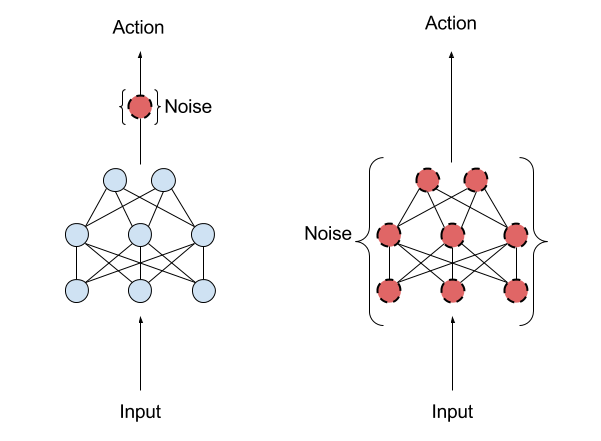
\includegraphics[width=0.8\textwidth]{./images/p_diag_1}
\caption{2 төрлийг орчны шуугиан}
\end{figure}

\subsection{Үйлдлийн орчны шуугиан}

Үйлдлийн орчны шуугиан гэдэг нь орчны шуугианыг үйлдэл дээр нэмэхийг хэлдэг. Үйлдлийн орчны шуугиан дотор бие биетэйгээ хамааралтай шуугиан, бие биенээсээ хамааралгүй шуугиан гэх 2 шуугианыг авч үзнэ.

\subsubsection{Бие биетэйгээ хамааралтай шуугиан}

Correlated noise буюу бие биенээсээ хамааралтай шуугианыг үүсгэхдээ Ornstein–Uhlenbeck-ын процессыг ашиглаж байгаа. Энэ процесс нь бие биетэйгээ хамааралтай шуугианыг үүсгэж өгч байгаа. Доорх графикт ямархуу тархац, савалгаатай шуугиан үүсгэж байгаа харууллаа. Хэвтээ тэнхлэгийн дагуу хэдэн удаа үүсгэсэн, босоо тэнхлэгийн дагуу ямар утга авах нь харгалзаж байна:

\begin{figure}[H]
\centering
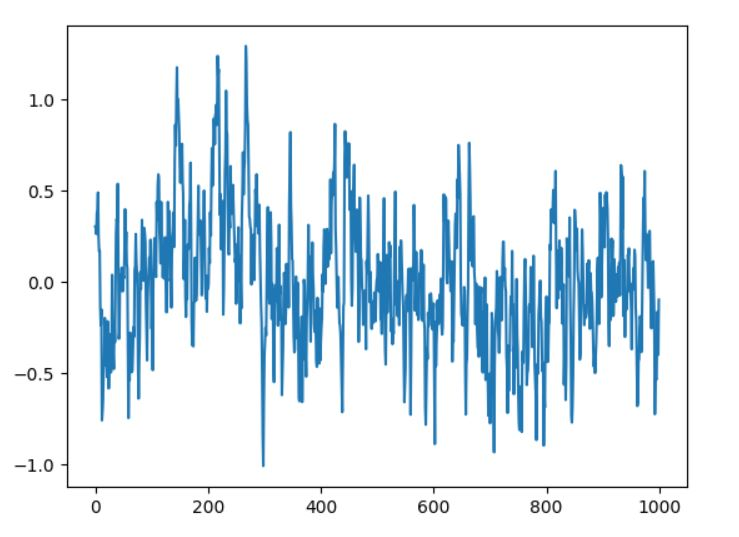
\includegraphics[width=0.8\textwidth]{./images/OU_process_graph}
\caption{OU процессын график}
\end{figure}

Туршилт хийхдээ хоёр өөр утга гаргах Ornstein–Uhlenbeck-ын процессын хэрэгжүүлэлтийг ашигласан. Нэг нь илүү тогтвортой алсуур аа савладаг, нөгөө тогтворгүй савлалт ихтэй байна. Доорх графикт ялгааг харууллаа:

\begin{figure}[H]
\centering
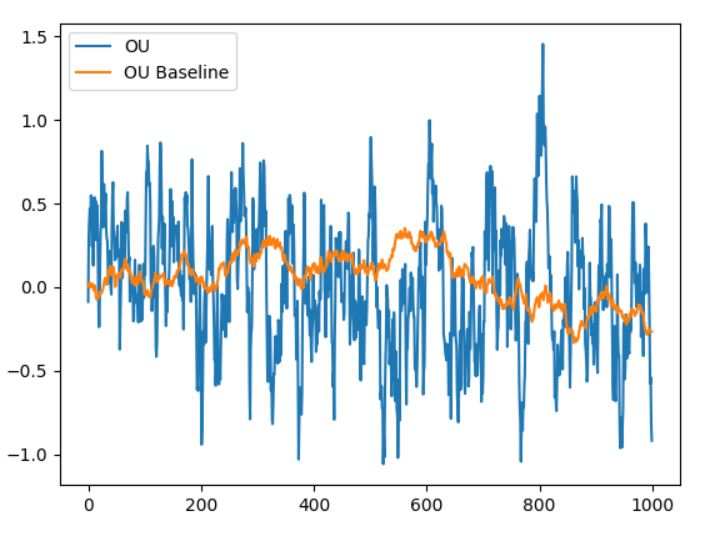
\includegraphics[width=0.8\textwidth]{./images/OU_OUBaseline_Graph}
\caption{2 өөр OU процессын график}
\end{figure}

\subsubsection{Бие биенээсээ хамааралгүй шуугиан}

Uncorrelated noise буюу бие биенээсээ хамааралгүй шуугианыг үүсгэхдээ [-0.2, 0.2]-ын хооронд санамсаргүй тоо авах байдлаар үүсгэж байгаа. Яагаад [-0.2, 0.2]-ын хооронд авч байгаа вэ гэхээр 3 төрлийн шуугианаа хооронд нь харьцуулах учраас адилхан параметртэй хэрэгжүүлж байгаа. Доорх графикт ямархуу тархац, савалгаатай шуугиан үүсгэж байгаа харууллаа (1000 удаа үүсгэсэн):

\begin{figure}[H]
\centering
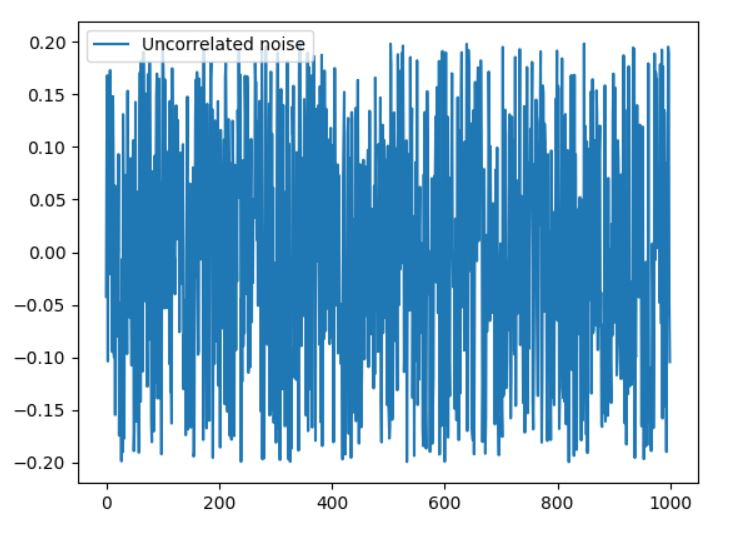
\includegraphics[width=0.8\textwidth]{./images/Uncorrelated_noise}
\caption{Бие биенээсээ хамааралгүй шуугианы график}
\end{figure}

\subsection{Параметр шуугиан}
 
Параметр шуугиан нь бусад аргуудаас илүү үр дүнтэй арга юм. Параметр шуугиан нь үйлдэлд шуугиан нэмэх бус неорал сүлжээн дээр параметр байдлаар шуугианыг нэмдэг. Шуугиан нь дасан зохицдог шуугиан (Adaptive noise) байна. Уламжлалт RL нь үйлдлийн орчны шуугианыг ашиглан агент нэг алхмаас нөгөө алхамд хийх үйлдэл бүртэй холбоотой магадлалыг өөрчилдөг. Параметр шуугиан нь алгоритмыг орчноо илүү үр дүнтэй судалж, илүү өндөр оноо авахад тусалдаг. [7]

\subsection{Параметр шуугианыг хэрэгжүүлэх}

Episode болгоны эхэнд actor сүлжээг хуулж аваад Гауссын шуугианыг нэмж шинэ шуугиантай actor сүлжээ үүсгэнэ.

\begin{center}
$\tilde{\theta}^Q=\theta^Q+N(0, \sigma^2)$
\end{center}

Тухайн episode шинэ үүссэн actor сүлжээн дээр сургагдана. Episode дууссаны дараа шинэ үүссэн actor сүлжээний үйлдлүүд болон энгийн actor сүлжээний үйлдлүүд хоорондын зай тооцно. Зайг тооцохдоо:

\begin{center}

$d(\theta^Q, \tilde{\theta^Q})=\sqrt{1/N\sum_{i=1}^{n}E_s[(\theta^Q(s)_i-\tilde{\theta^Q(s)_i})^2]}),$

\end{center}

N = үйлдлийн хэмжээс

Шинэ үүссэн actor сүлжээний үйлдлүүд болон энгийн actor сүлжээний үйлдлүүд хоорондын зөрүүний квадратуудын нийлбэрийг олоод үүний язгуурыг олж байна.

Энэ нь ямар байгаагаас хамааран параметр шуугианыхаа сигмаг өөрчилнө:

\begin{center}
\[ \sigma_{k+1} =
  \begin{cases}
    \alpha\sigma_k       & \quad \text{Хэрвээ } d(\theta^Q, \tilde{\theta^Q})\leq\delta,\\
    \frac{1}{\alpha}\sigma_k  & \quad \text{Бусад тохиолдолд },
  \end{cases}
\]
\end{center}

Дээрх байдлаар шуугианыхаа $\sigma$-г өөрчилөн явна. Ийм байдлаар хэрэгжүүлэлтийг хийх болно.

\subsubsection{Off-policy аргад зориулсан параметер шуугиан}

Off-policy үед суралцах үйл явцыг (exploration) шинэ үүсгэсэн actor сүлжээн дээр хийх бөгөөд сургах процессоо энгийн actor сүлжээн дээрээ хийнэ.

\section{Ашигласан технологи}

\subsection{Gym}

Gym бол reinforcement learning буюу бататгасан сургалтын алгоритмуудыг хөгжүүлэх болон харьцуулахад зориулагдсан хэрэгсэл юм. Үүнийг ашиглан агентдаа алхах, тоглоом тоглох зэрэг бүх зүйлийг зааж болно. 

\subsubsection{Яагаад үүнийг ашигладаг вэ?}

Бататгасан сургалт (RL) нь шийдвэр гаргахтай холбоотой машин сургалтын дэд талбар юм. Энэ нь агент нарийн төвөгтэй, тодорхойгүй орчинд хэрхэн зорилгодоо хүрч болохыг судалдаг. RL нь доорх 2 шалтгааны улмаас ихээр ашиглагдаж байна:

\begin{itemize}
	\item RL нь дараалсан шийдвэр гаргахтай холбоотой бүхий л асуудлыг багтаасан байдаг. Жишээ нь роботын хөдөлгүүрийг удирдаж түүнийг үсрэх чадвартай болгох, үнэ, бараа материалын менежмент гэх мэт бизнесийн шийдвэр гаргах, видео тоглоом, ширээний тоглоом тоглох гэх мэт
	\item RL алгоритмууд олон хүнд хэцүү орчинд сайн үр дүнд хүрч эхэлсэн
\end{itemize} 

Гэсэн хэдий ч RL судалгааны ажлыг RL-ын open-source орчин хангалттай олон янз байдаггүй бөгөөд тэдгээрийг тохируулах, ашиглахад хэцүү байдал болон орчны стандартчилал дутмаг гэсэн хоёр хүчин зүйл удаашруулж байна. Gym нь эдгээр 2 асуудлыг шийдэхийг зоридог.

\subsection{BiPedalWalker-v2}

Энэ бол gym-ын Box2D симулятор дахь нэг орчин юм. Гол зорилго нь bipedal роботыг алхаж сургах. Урагш алхах бүрд reward өгдөг. Нийтдээ төгсгөл хүртэл 300+ оноог өгдөг. Хэрэв робот унавал -100 оноо өгдөг. Илүү сайн агент нь илүү сайн оноо авах болно. 

Төлөв нь их биений өнцгийн хурд, өнцгийн хурд, хэвтээ хурд, босоо хурд, хөлний байрлал, хөлний өнцгийн хурд, хөлтэй газар шүргэлцэх, 10 лидарын зай хэмжигч хэмжигдэхүүнээс бүрдэнэ. Мужийн векторт координат байхгүй байна.

\subsection{Pytorch}

Pytorch бол Torch сан дээр тулгуурласан open-source машин сургалтын сан юм. Python хэлэнд ихээр ашиглагддаг ч мөн С++ програмчлалын хэлд ашиглагддаг. Энэ нь GPU ашигладаг. PyTorch нь өндөр түвшний хоёр онцлог шинж чанарыг агуулдаг:

\begin{itemize}
	\item GPU-г ашиглан тензорын тооцоолол хийх (NumPy гэх мэт) 
	\item Гүнзгий неороны сүлжээг (Deep neural network) бий болгох
\end{itemize}

2016 оны 1 сард гарсан бөгөөд үүнээс хойш олон судлаачид үүнийг ашигласаар байна. Учир нь маш нарийн төвөгтэй неороны сүлжээг хялбараар бий болгодог. Мөн кодоо шалгахдаа заавал бүхлээр нь ажиллуулах шаардлагагүй болсон. Шаардлагатай тохиолдолд Pytorch-ын функцуудыг NumPy, SciPy, Cython зэргээр өргөтгөж болно. 
 
\chapter{Хэрэгжүүлэлт}

\section{Алгоритмын хэрэгжүүлэлт}

Хэрэгжүүлэлтийг python програмчлалын хэлийг ашиглан гүйцэтгэсэн. Орчинг бэлдэхдээ gym openai хэрэгслийг ашигласан. Pytorch санг тооцоолол хийх, неороны сүлжээ үүсгэх зэрэгт ашигласан. Дээр дурдсан DDPG алгоритмын pseudo кодын дагуу кодыг бичсэн. 3 шуугианы гүйцэтгэлийг харьцуулах учраас ойролцоо хипер параметрүүдийг ашигласан.

DDPG алгоритмын хувьд Lillicrap et al.(2015)[4]-дээр тайлбарласантай төстэй actor, critic сүлжээний архитектурыг ашигласан. Target сүлжээнүүдийг $\tau=0.001$ гэсэн параметртэй soft-update хийсэн. Actor, critic сүлжээ хоёулаа Adam сургагчийг ашигласан.

Кодыг хавсралт хэсэг оруулсан. Github-аас харахыг хүсвэл дараах холбоосоор хандана уу \url{https://github.com/bbyambanyam/ddpg_algorithm.git}

\section{Алгоритмын турших орчин}

BipedalWalker-v3 орчин дээр алгоритмыг ажиллуулан туршилаа.

\begin{figure}[H]
\centering
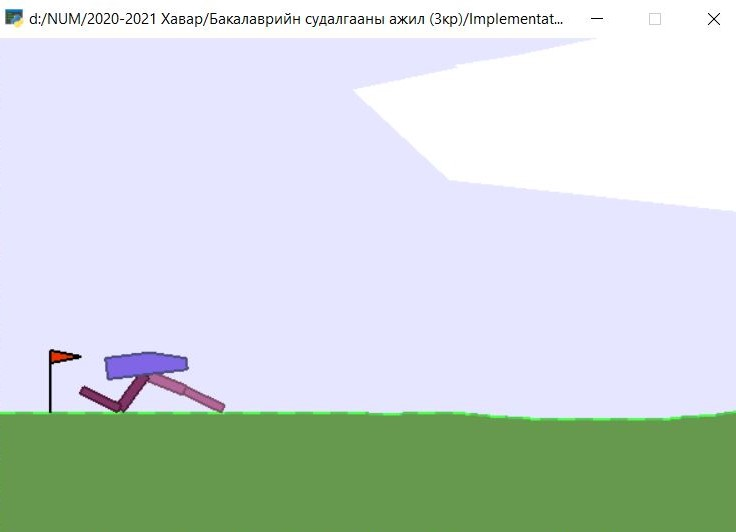
\includegraphics[width=0.8\textwidth]{./images/bipedalwalker}
\caption{BiPedalWalker-V3 орчин}
\end{figure}

Орчинг үүсгэж төлөвийн хэмжээс, үйлдлийн хэмжээс, хийж болох үйлдлийн тоог авна.

\begin{lstlisting}[language=Python, caption=Орчин үүсгэх, frame=single]
env = gym.make('BipedalWalker-v3')

state_dimension = env.observation_space.shape[0]
action_dimension = env.action_space.shape[0]
action_max = env.action_space.high[0]
\end{lstlisting}

\subsection{Хипер параметрүүд}

Доорх DDPG-ийн хипер параметрүүд нь BiPedalWalker-V3 орчныг шийдвэрлэхэд тохируулагдсан болно. Зарим тохиолдолд өөр байж болно.

\begin{itemize}
	\item Actor learning rate: 0.0001 (Adam optimizer)
	\item Critic learning rate: 0.001 (Adam optimizer)
	\item Memory buffer size: 1000000
	\item Minibatch size: 128
	\item OU-noise-theta: 0.15
	\item OU-noise-sigma: 0.2
	\item OU-noise-mu: 0
	\item normal-noise: 0.2
	\item Steps: 1600
	\item Target update: 0.001
	\item initial-stddev ($\sigma$): 0.1
	\item desired-action-stddev ($\delta$): 0.2
	\item adaptation-coefficient($\alpha$): 1.01
\end{itemize}

\section{Чухал кодын хэсгүүд}

Actor, target actor, critic болон target critic сүлжээг optimizer (сургагч)-ын хамт үүсгэх. Үүсгэхдээ төлөвийн хэмжээс, үйлдлийн хэмжээс, хийж болох үйлдлийн тоо зэргийг ашиглана.

\begin{lstlisting}[language=Python, caption=Actor critic сүлжээ үүсгэх, frame=single]
actor = models.Actor(state_dimension, action_dimension, action_max)
target_actor = models.Actor(state_dimension, action_dimension, action_max)
actor_optimizer = torch.optim.Adam(actor.parameters(), lr=0.001)

critic = models.Critic(state_dimension, action_dimension)
target_critic = models.Critic(state_dimension, action_dimension)
critic_optimizer = torch.optim.Adam(critic.parameters(), lr=0.001)

for target_param, param in zip(target_actor.parameters(), actor.parameters()):
	target_param.data.copy_(param.data)

for target_param, param in zip(target_critic.parameters(), critic.parameters()):
    target_param.data.copy_(param.data)
\end{lstlisting}

Replay buffer үүсгэх. Buffer-аа үүсгэснийхээ дараа hot start хийхийн тулд санамсаргүй утгуудаар дүүргэж өгсөн.

\begin{lstlisting}[language=Python, caption=Replay buffer үүсгэх, frame=single]
ram = memory.ReplayBuffer(1000000))
\end{lstlisting}

Ornstein-Uhlenbeck Process-г үүсгэх

\begin{lstlisting}[language=Python, caption=Шуугиан үүсгэх, frame=single]
noise = utilities.OrnsteinUhlenbeckActionNoise(action_dimension)
\end{lstlisting}

Дээр үүсгэсэн шуугианаа ашиглан үйлдэл дээр correleted шуугианыг нэмэх

\begin{lstlisting}[language=Python, caption=Үйлдэл дээр шуугиан нэмэх, frame=single]
action_with_noise = action_without_noise.data.numpy() + (noise.sample() * action_max)
\end{lstlisting}

Үйлдэл дээр uncorreleted шуугианыг нэмэх

\begin{lstlisting}[language=Python, caption=Үйлдэл дээр шуугиан нэмэх, frame=single]
action_with_noise = action_without_noise.data.numpy() + (random.uniform(-0.2, 0.2) * action_max)
\end{lstlisting}

Параметр шуугиан үүсгэх

\begin{lstlisting}[language=Python, caption=Үйлдэл дээр шуугиан нэмэх, frame=single]
#Parameter noise-d zoriulsan actor
actor_copy = models.Actor(state_dimension, action_dimension, action_max)

#Parameter noise
parameter_noise = utilities.AdaptiveParamNoiseSpec(initial_stddev=0.05,desired_action_stddev=0.3, adaptation_coefficient=1.05)
\end{lstlisting}

Параметр шуугианд зориулан үүсгэсэн шинэ actor сүлжээний неорал сүлжээн дээр параметр шуугианыг нэмэх

\begin{lstlisting}[language=Python, caption=Үйлдэл хийх, frame=single]
parameters = actor_copy.state_dict()
for name in parameters:
    parameter = parameters[name]
    rand_number = torch.randn(parameter.shape)
    parameter = parameter + rand_number * parameter_noise.current_stddev
\end{lstlisting}

Үйлдлийг хийж шинэ төлөв, reward-г авах

\begin{lstlisting}[language=Python, caption=Үйлдэл хийх, frame=single]
new_observation, reward, done, info = env.step(action_with_noise)
\end{lstlisting}

Параметр шуугианы зай тооцох, сигмаг шинэчлэх

\begin{lstlisting}[language=Python, caption=Үйлдэл хийх, frame=single]
#Distance tootsoh
diff_actions = actor_copy_actions - actor_actions
mean_diff_actions = np.mean(np.square(diff_actions),axis=0)
distance = math.sqrt(np.mean(mean_diff_actions))

#Sigma-g update hiih
parameter_noise.adapt(distance)
\end{lstlisting}

Critic сүлжээг сургаад, шинэчлэх

\begin{lstlisting}[language=Python, caption=Critic сүлжээг сургах шинэчлэх, frame=single]
# Critic network-g surgah

predicted_action = target_actor.forward(next_states).detach()
next_val = torch.squeeze(target_critic.forward(next_states, predicted_action).detach())
y_expected = rewards + 0.99*next_val
y_predicted = torch.squeeze(critic.forward(states, actions))

# Critic network-g shinechleh, critic loss-g tootsooloh
            
critic_loss = F.smooth_l1_loss(y_predicted, y_expected)
critic_optimizer.zero_grad()
critic_loss.backward()
critic_optimizer.step()
\end{lstlisting}	

Actor сүлжээг сургах

\begin{lstlisting}[language=Python, caption=Actor сүлжээг сургах, frame=single]
predicted_action = actor.forward(states)
actor_loss = -1*torch.sum(critic.forward(states, predicted_action))
actor_optimizer.zero_grad()
щactor_loss.backward()
щactor_optimizer.step()
\end{lstlisting}

\chapter{Үр дүнгийн боловсруулалт}

\section{Туршилтын үр дүн}

Хэрэв алгоритм зөв ажиллаж байгаа бол reward нь өсөж байх ёстой байдаг. Дундаж reward-ыг авахдаа episode болгоны нийлбэр reward-г олоод үүнийгээ list-д хадгалан аваад энэ list-ээс сүүлийн 40 үр дүнгийн дундажыг олж графикийг зурсан.

\subsection{Үйлдлийн орчны шуугиан}

\subsubsection{Correlated шуугиан}

Доорх графикийн хувьд 800 episode ажилласан бөгөөд босоо тэнхлэгийн дагуу дундаж reward, хэвтээ тэнхлэгийн дагуу ажилласан episode-г авч байна. Орчны шуугианыг нэмэхдээ Ornstein-Uhlenbeck Process-г ашигласан. Доорх бүх графикийн хувьд Actor LEARNING RATE: 0.001 Critic LEARNING RATE: 0.001 бусад хипер параметрүүд ижил.

\begin{figure}[H]
\centering
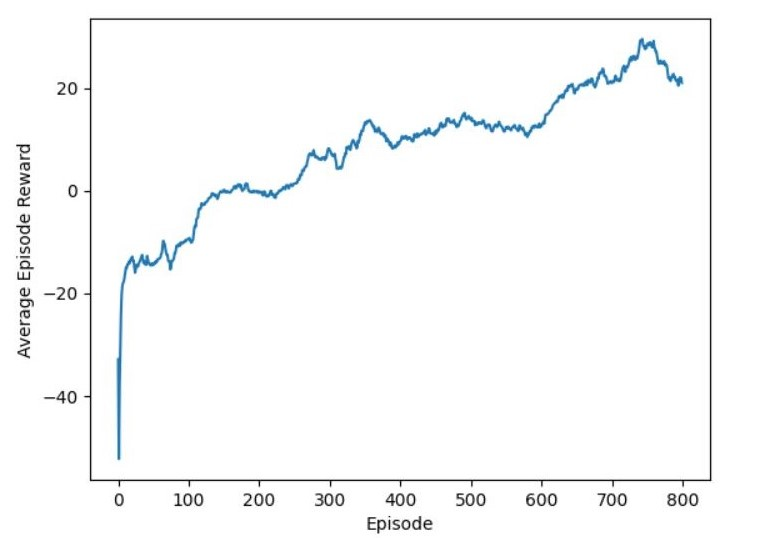
\includegraphics[width=0.7\textwidth]{./images/after_800_ep}
\caption{Correlated noise}
\end{figure}

1000 episode ажиллуулсны дараа:

\begin{figure}[H]
\centering
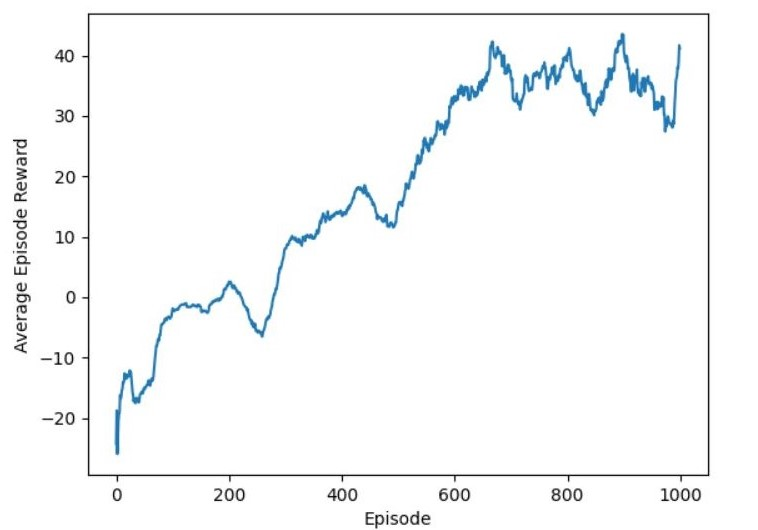
\includegraphics[width=0.7\textwidth]{./images/after_1000_ep2}
\caption{Correlated noise}
\end{figure}

\subsubsection{Uncorrelated шуугиан}

Доорх хоёр графикийн хувьд 800 episode ажилласан бөгөөд орчны шуугианыг -0.2 оос 0.2-ын хооронд санамсаргүй байдлаар сонгон авч үйлдэл дээрээ нэмж байгаа. Энэ нь өмнөх шуугиантай уялдаа хамааралгүй буюу uncorrelated шуугиан гэсэн үг юм. Доорх бүх грапикийн хувьд Actor LEARNING RATE: 0.001 Critic LEARNING RATE: 0.001 бусад хипер параметрүүд ижил. 

\begin{figure}[H]
\centering
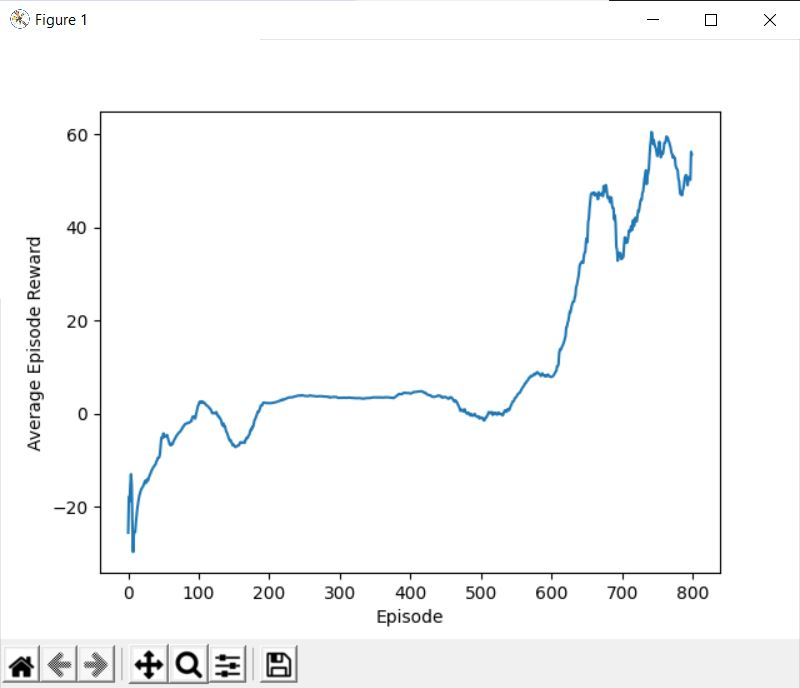
\includegraphics[width=0.7\textwidth]{./images/after_800_ep_02}
\caption{Uncorrelated noise}
\end{figure}

Uncorreleted шуугианы өөр нэг график:

\begin{figure}[H]
\centering
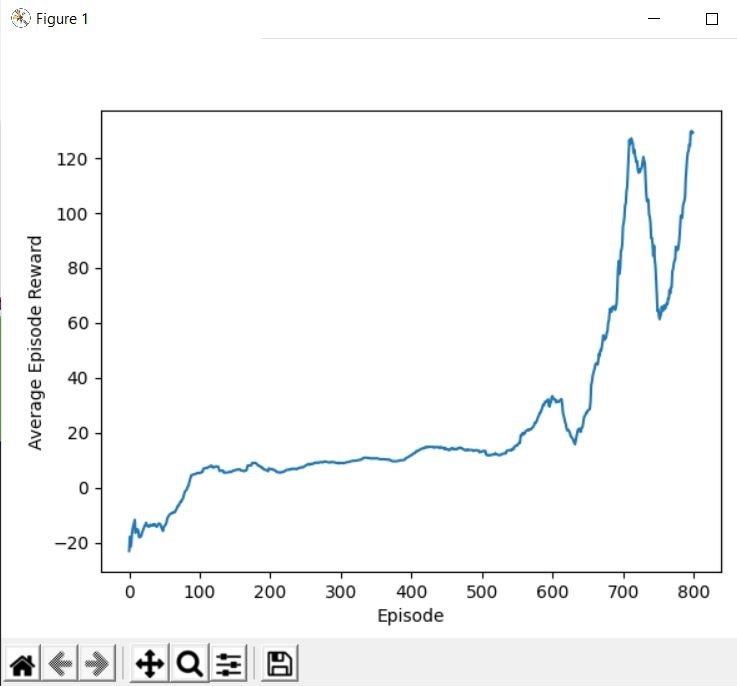
\includegraphics[width=0.7\textwidth]{./images/after_800_ep_02_am}
\caption{Uncorrelated noise 2}
\end{figure}

Доорх графикийн хувьд 800 episode ажилласан бөгөөд орчны шуугианыг -0.4-оос 0.4-ын хооронд санамсаргүй байдлаар сонгон авч үйлдэл дээрээ нэмж байгаа. Энэ нь мөн адил өмнөх шуугиантай уялдаа хамааралгүй буюу uncorrelated шуугиан юм. Графикаас харахад 0.4 өөр сонгон авсан үед нь үр дүн муу гарч байна.

\begin{figure}[H]
\centering
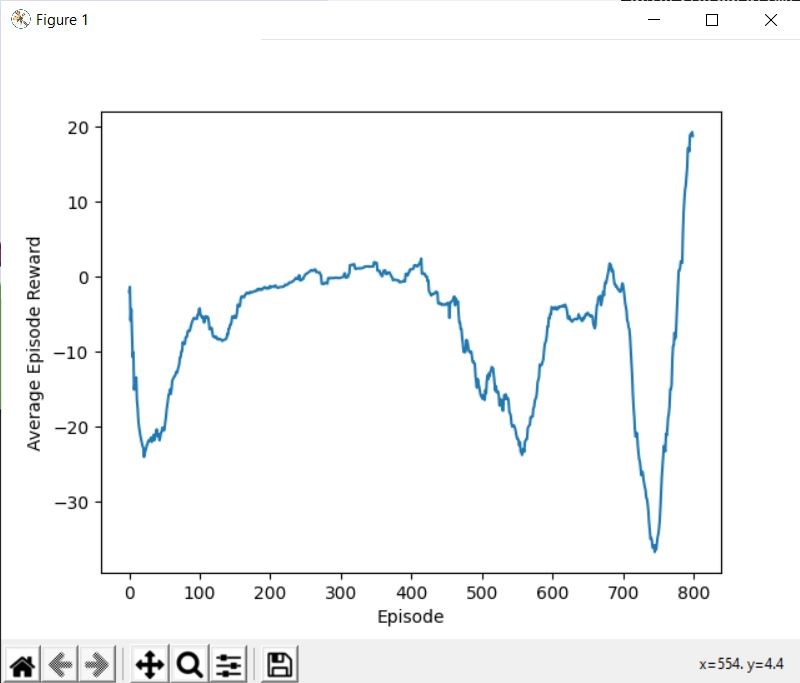
\includegraphics[width=0.8\textwidth]{./images/after_800_ep_04}
\caption{Uncorrelated noise 0.4}
\end{figure}

\subsection{Parameter Space Noise}

Доорх параметр шуугианы үр дүнг нь гаргахын тулд 1200 episode ажиллуулсан. ACTOR LEARNING RATE: 0.0001, CRITIC LEARNING RATE: 0.001:

\begin{figure}[H]
\centering
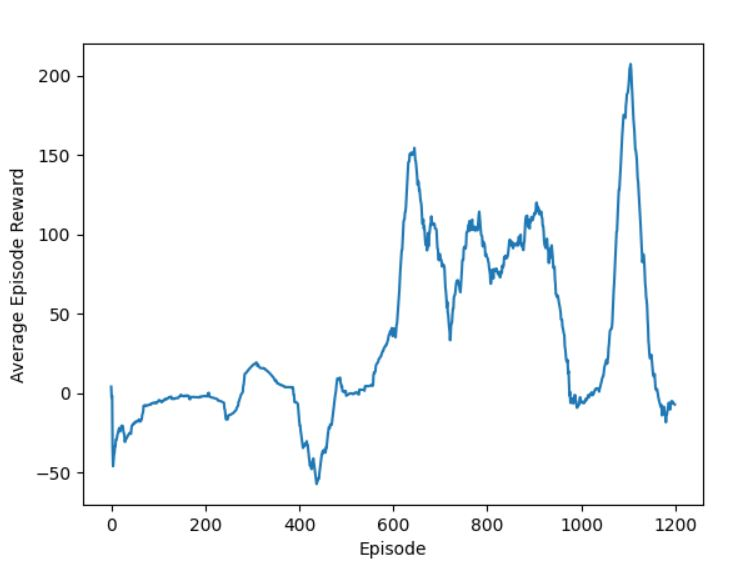
\includegraphics[width=0.8\textwidth]{./images/PSN_a-lr-0-0001_c-lr-0-001_1200ep}
\caption{Параметр орчны шуугиан}
\end{figure}

\section{Үр дүнгийн харьцуулалт}

Харьцуулалт хийхийн тулд бүх шуугиан дээр ижил хипер параметртэйгээр ажиллуулсан.  Uncorrelated noise буюу бие биенээсээ хамааралгүй шуугиан ($\theta=0, \sigma=0.2$), Correlated noise буюу бие биетэйгээ хамааралтай шуугиан (Ornstein–Uhlenbeck process), Parameter space noise буюу параметр шуугиан гэсэн гурван шуугианы харьцуулалтыг хийлээ. Мөн үр дүнг хоорондоо харьцуулагдах боломжтой болгохын тулд параметр шуугианыг дангаар нь ашиглахгүйгээр Ornstein-Uhlenbeck-ын процесстой цуг ашигласан.

Доорх графикийн хувьд үр дүнг гаргахдаа 101 episode ажиллуулсан бөгөөд нэг episode-д хийх алхам буюу MAX-STEP нь 10000 байна. Гүйцэтгэлийг үнэлэхийн тулд эхний 20 episode-ыг ямар ч шуугиангүйгээр ажиллуулсан. 

\begin{figure}[H]
\centering
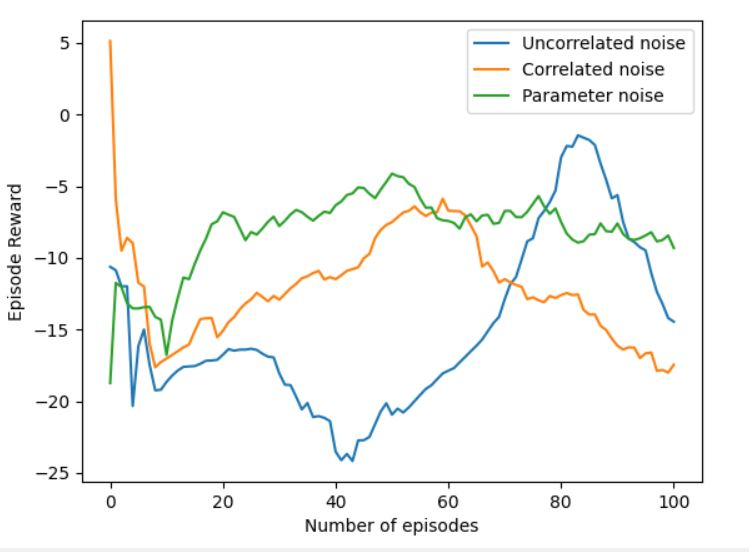
\includegraphics[width=0.8\textwidth]{./images/comperation-3}
\caption{Харьцуулалтын грапик}
\end{figure}

Графикаас харахад бие биенээсээ хамааралгүй шуугианы хувьд савалгаа ихтэй байгаа нь харагдаж байна. Дундаж шагнал нь episode 80 дээр их хэмжээтэй гарч байгаа ч савалгаа их тул буурах шинжтэй байна. Бие биетэйгээ хамааралтай шуугианы хувьд савалгаа дундаж байгаа ч дундаж шагналын хувьд харьцангуй бага байна. Параметр шуугианы хувьд  савалгаа маш бага дундаж шагнал нь бага байна. Үүнээс дүгнэхэд гүйцэтгэлийн хувьд параметр шуугиан нь маш бага зэрэг илүү байна. Мөн үүнийг батлах өөр нэг үр дүн бол Зураг 3.6 бөгөөд уг зурагт дундаж шагналын хамгийн дээд хэмжээ нь 200+ байна. Бусад шуугианы хувьд дундаж шагнал ийм хэмжээнд хүрээгүй. BipedalWalker-V3 орчин дээр роботын алхах чадварын хувьд параметр шуугианы хувьд илүү байсан. Гэхдээ параметр шуугианы хувьд илт давуу сайн биш байгаа бөгөөд хүлээлтэд хүрээгүй үр дүн гарсан нь хэрэгжүүлэлтийн үед алдаа гарсан байж болзошгүй эсвэл хипер параметрүүд сайн таараагүй гэж харж байна.

%----------------------------------------------------------------------------------------
%   Дүгнэлт эндээс эхэлнэ
%----------------------------------------------------------------------------------------
\conclusion{Дүгнэлт}

Энэхүү судалгааны ажлаар 3 төрлийн шуугианыг DDPG алгоритмыг ашиглан BipedalWalker-V3 орчин дээр амжилттай туршиж гүйцэтгэлээ. Бие биенээсээ хамааралгүй болон бие биетэйгээ хамааралтай шуугианы хувьд үр дүнг хангалттай сайн гарсан гэж харж байгаа бол параметр шуугианы хувьд үр дүн хангалттай сайн сайн биш ч бүр муу үр дүн гараагүй гэж харж байна. Үр дүнгээс үзэхэд шуугианыг нэмэх хамгийн сайн арга бол үйлдэлд шууд шуугиан нэмэх бус неорал сүлжээнд параметр байдлаар шуугианыг нэмэх нь илүү гэдгийг харж болохоор байна. Роботын алхах чадвараас харахад параметр шуугиан нь орчны асуудлыг илүү сайн шийдвэрлэж чадаж байгааг харж болохоор байсан. 

Хэрэгжүүлэлтийн явцад гаргасан нэг алдаа бол сургасан моделиудаа хадгалдаг, хадгалсан моделио уншиж аваад үргэлжлүүлэн сургадаг үйлдлийг параметр шуугианыг хэрэгжүүлснийхээ дараа хийх бус анх DDPG алгоритмаа хэрэгжүүлэхдээ цуг хийх байсан юм. Үүнийг эрт хэрэгжүүлээгүйгээс болж бие биенээсээ хамааралгүй шуугиан болон бие биетэйгээ хамааралтай шуугианы моделийг хадгалан аваагүй учир харьцуулалт хийхэд энэ хоёр шуугианыг дахин сургах асуудал гарсан.

%----------------------------------------------------------------------------------------
%   Дипломын номзүй, хавсралтын хэсэг эндээс эхэлнэ
%----------------------------------------------------------------------------------------

\singlespace
\addcontentsline{toc}{part}{НОМ ЗҮЙ}
\begin{thebibliography}{}
	% Ашигласан материалыг эндээс оруулна
	\bibitem{image1}
	Deep Deterministic Policy Gradients Explained, TowardsDataScience, \url{https://towardsdatascience.com/deep-deterministic-policy-gradients-explained-2d94655a9b7b}
	\bibitem{pharagraph1}
	Deep Deterministic Policy Gradient (DDPG),  Keras, \url{https://keras.io/examples/rl/ddpg_pendulum/}
	\bibitem{format1}
	Deep Deterministic Policy Gradient, Spinning Up, \url{https://spinningup.openai.com/en/latest/algorithms/ddpg.html}
	\bibitem{list}
	Continuous Control With Deep Reinforcement Learning, Lillicrap et al 2015, \url{https://arxiv.org/pdf/1509.02971.pdf}
	\bibitem{Parameter noise}
	Parameter noise,  Openai, \url{https://openai.com/blog/better-exploration-with-parameter-noise/}
	\bibitem{Evolution stratagies}
	Evolution stratagies,  Openai, \url{https://openai.com/blog/evolution-strategies/}
	\bibitem{Parameter}
	Parameter space noise for exploration,  Arxiv, \url{https://arxiv.org/abs/1706.01905}
	
	\bibitem{list}
	Benchmarking Deep Reinforcement Learning for Continuous Control,  Arxiv, \url{https://arxiv.org/abs/1604.06778}
	\bibitem{Benchmark}
	Policy Gradient Algorithms. 2018.,  LilianWeng, \url{https://lilianweng.github.io/lil-log/2018/04/08/policy-gradient-algorithms.html}
	
\end{thebibliography}


%----------------------------------------------------------------------------------------
%   Хавсралтууд эндээс эхэлнэ
%----------------------------------------------------------------------------------------
\appendix
\addcontentsline{toc}{part}{ХАВСРАЛТ}

% Хавсралтын нэр. Хавсралт гэдэг үг агуулахгүй
\chapter{Кодын хэрэгжүүлэлт}

\begin{lstlisting}[language=Python, caption=models.py, frame=single]
import torch
import torch.nn as nn
import torch.nn.functional as F
import numpy as np

def fanin_init(size, fanin=None):
    fanin = fanin or size[0]
    v = 1. / np.sqrt(fanin)
    return torch.Tensor(size).uniform_(-v, v)

class Actor(nn.Module):
    def __init__(self, state_dimension, action_dimension, action_max):
        super(Actor, self).__init__()

        self.state_dimension = state_dimension
        self.action_dimension = action_dimension
        self.action_max = action_max

        # 3 layer uusgene

        self.fc1 = nn.Linear(state_dimension, 256)
        self.fc2 = nn.Linear(256, 128)
        self.fc3 = nn.Linear(128, 64)
        self.fc4 = nn.Linear(64, action_dimension)
        
        self.fc1.weight.data = fanin_init(self.fc1.weight.data.size())
        self.fc2.weight.data = fanin_init(self.fc2.weight.data.size())
        self.fc3.weight.data = fanin_init(self.fc3.weight.data.size())
        self.fc4.weight.data.uniform_(-0.003, 0.003)

    def forward(self, state):
        output = self.fc1(state)
        output = F.relu(output)

        output = self.fc2(output)
        output = F.relu(output)

        output = self.fc3(output)
        output = F.relu(output)

        action = self.fc4(output)
        action = F.tanh(action)

        action = action * self.action_max

        # action butsaana

        return action

class Critic(nn.Module):
    def __init__(self, state_dimension, action_dimension):
        super(Critic, self).__init__()

        self.state_dimension = state_dimension
        self.action_dimension = action_dimension
        
        # 4 layer uusgene

        self.fcs1 = nn.Linear(state_dimension, 256)
        self.fcs2 = nn.Linear(256, 128)
        self.fca1 = nn.Linear(action_dimension, 128)
        self.fc2 = nn.Linear(256, 128)
        self.fc3 = nn.Linear(128, 1)

        self.fcs1.weight.data = fanin_init(self.fcs1.weight.data.size())
        self.fcs2.weight.data = fanin_init(self.fcs2.weight.data.size())
        self.fca1.weight.data = fanin_init(self.fca1.weight.data.size())
        self.fc2.weight.data = fanin_init(self.fc2.weight.data.size())
        self.fc3.weight.data.uniform_(-0.003, 0.003)

    def forward(self, state, action):
        s1 = self.fcs1(state)
        s1 = F.relu(s1)
        s2 = self.fcs2(s1)
        s2 = F.relu(s2)
        a1 = self.fca1(action)
        a1 = F.relu(a1)

        output = torch.cat((s2, a1), dim=1)
        output = self.fc2(output)
        output = F.relu(output)
        q_value = self.fc3(output)

        # Q value-g butsaana

        return q_value
\end{lstlisting}

\begin{lstlisting}[language=Python, caption=memory.py, frame=single]
import numpy as np
from collections import deque
import random

# experience-uudiig hadgalah buffer

class ReplayBuffer:
    def __init__(self, size):
        self.size = size
        self.buffer = deque(maxlen=self.size)

    # experience-g buffer-t nemeh

    def add(self, state, action, reward, next_state):
        exp = (state, action, reward, next_state)
        self.buffer.append(exp)

    # Randor-oor size-toonii experience-g awah

    def sample_exp(self, size):
        batch = []
        size = min(size, len(self.buffer))
        batch = random.sample(self.buffer, size)
        
        states = np.float32([arr[0] for arr in batch])
        actions = np.float32([arr[1] for arr in batch])
        rewards = np.float32([arr[2] for arr in batch])
        next_states = np.float32([arr[3] for arr in batch])
        
        return states, actions, rewards, next_states
\end{lstlisting}

\begin{lstlisting}[language=Python, caption=utilities.py, frame=single]
import numpy as np

#Ornstein-uhlenbeck process-g correlated noise uusgehed ashiglana

#http://math.stackexchange.com/questions/1287634/implementing-ornstein-uhlenbeck-in-matlab

class OrnsteinUhlenbeckActionNoise:

	def __init__(self, action_dim, mu = 0, theta = 0.15, sigma = 0.2):
		self.action_dim = action_dim
		self.mu = mu
		self.theta = theta
		self.sigma = sigma
		self.X = np.ones(self.action_dim) * self.mu

	def reset(self):
		self.X = np.ones(self.action_dim) * self.mu

	def sample(self):
		dx = self.theta * (self.mu - self.X)
		dx = dx + self.sigma * np.random.randn(len(self.X))
		self.X = self.X + dx
		return self.X

class ActionNoise(object):
    def reset(self):
        pass

#Based on https://github.com/openai/baselines/tree/master/baselines/ddpg
class OrnsteinUhlenbeckActionNoiseBaseline(ActionNoise):
    def __init__(self, mu, sigma, theta=.15, dt=1e-2, x0=None):
        self.theta = theta
        self.mu = mu
        self.sigma = sigma
        self.dt = dt
        self.x0 = x0
        self.reset()

    def __call__(self):
        x = self.x_prev + self.theta * (self.mu - self.x_prev) * self.dt + self.sigma * np.sqrt(self.dt) * np.random.normal(size=self.mu.shape)
        self.x_prev = x
        return x

    def reset(self):
        self.x_prev = self.x0 if self.x0 is not None else np.zeros_like(self.mu)

    def __repr__(self):
        return 'OrnsteinUhlenbeckActionNoise(mu={}, sigma={})'.format(self.mu, self.sigma)

class AdaptiveParamNoiseSpec(object):
    def __init__(self, initial_stddev=0.1, desired_action_stddev=0.2, adaptation_coefficient=1.01):
        self.initial_stddev = initial_stddev
        self.desired_action_stddev = desired_action_stddev
        self.adaptation_coefficient = adaptation_coefficient

        self.current_stddev = initial_stddev

    def adapt(self, distance):
        if distance > self.desired_action_stddev:
            # Decrease stddev.
            self.current_stddev /= self.adaptation_coefficient
        else:
            # Increase stddev.
            self.current_stddev *= self.adaptation_coefficient

    def get_stats(self):
        stats = {
            'param_noise_stddev': self.current_stddev,
        }
        return stats

    def __repr__(self):
        fmt = 'AdaptiveParamNoiseSpec(initial_stddev={}, desired_action_stddev={}, adaptation_coefficient={})'
        return fmt.format(self.initial_stddev, self.desired_action_stddev, self.adaptation_coefficient)

if __name__ == '__main__':
    ou = OrnsteinUhlenbeckActionNoise(1)
    ou_baseline = OrnsteinUhlenbeckActionNoiseBaseline(mu=np.zeros(1), sigma=float(0.2) * np.ones(1))
    
    states = []
    states2 = []
    
    for i in range(1000):
        states.append(ou.sample())
        states2.append(ou_baseline())
	
    import matplotlib.pyplot as plt
    
    plt.plot(states, label = "OU")
    plt.plot(states2, label = "OU Baseline")
    plt.legend()
    plt.show()

\end{lstlisting}

\begin{lstlisting}[language=Python, caption=main.py, frame=single]
import gc
import random
import gym
import numpy as np
import matplotlib.pyplot as plt
from torch.autograd import Variable
import torch
import torch.nn.functional as F
import pickle
import os
import math
import time

import memory
import models
import utilities

if __name__ == "__main__":

    ACTOR_LEARNING_RATE = 0.0001
    CRITIC_LEARNING_RATE = 0.001
    MAX_EPISODE = 1201
    MAX_STEPS = 1600
    NOISE_TYPE = "ParameterWithOU" #OU, OUBaseline, Parameter, Uncorrelated, NoNoise, ParameterWithOU
    # Orchin beldeh
    env = gym.make('BipedalWalker-v3')

    state_dimension = env.observation_space.shape[0]
    action_dimension = env.action_space.shape[0]
    action_max = env.action_space.high[0]

    print("State dimension: {}" .format(state_dimension))
    print("Action dimension: {}" .format(action_dimension))
    print("Action max: {}" .format(action_max))

    load_models = False

    # Actor network, critic network uusgeh

    actor = models.Actor(state_dimension, action_dimension, action_max)
    target_actor = models.Actor(state_dimension, action_dimension, action_max)
    actor_optimizer = torch.optim.Adam(actor.parameters(), lr=ACTOR_LEARNING_RATE)

    critic = models.Critic(state_dimension, action_dimension)
    target_critic = models.Critic(state_dimension, action_dimension)
    critic_optimizer = torch.optim.Adam(critic.parameters(), lr=CRITIC_LEARNING_RATE)

    # Target network-g huulah

    for target_param, param in zip(target_actor.parameters(), actor.parameters()):
        target_param.data.copy_(param.data)

    for target_param, param in zip(target_critic.parameters(), critic.parameters()):
        target_param.data.copy_(param.data)

    # Hadgalsan modeliig ashiglah

    if load_models:
        actor.load_state_dict(torch.load('./Models/' + str(0) + '_actor.pt'))
        critic.load_state_dict(torch.load('./Models/' + str(0) + '_critic.pt'))

        for target_param, param in zip(target_actor.parameters(), actor.parameters()):
            target_param.data.copy_(param.data)

        for target_param, param in zip(target_critic.parameters(), critic.parameters()):
            target_param.data.copy_(param.data)

        print("Models loaded!")

    # Replay buffer uusgeh

    ram = memory.ReplayBuffer(1000000)

    #Buffer-g utgaar duurgeh (hot start)

    st = np.float32(env.reset())
    print(type(st))
    for step in range(128):
        action = env.action_space.sample()
        new_observation, reward, done, info = env.step(action)

        # Replay buffer-d state, action, reward, new_state -g hadgalah

        ram.add(st, action, reward, new_observation)

        if done:
            st = env.reset()
        else:
            st = new_observation

    print("Initial ram size: ", len(ram.buffer))

    # Reward-iig hadgalah list

    reward_list = []
    average_reward_list = []
    steps_reward_list = []

    # Noise uusgeh

    if NOISE_TYPE == "OU":
        noise = utilities.OrnsteinUhlenbeckActionNoise(action_dimension)
    elif NOISE_TYPE == "OUBaseline":
        noise = utilities.OrnsteinUhlenbeckActionNoiseBaseline(mu=np.zeros(action_dimension), sigma=float(0.2))
    elif NOISE_TYPE == "Parameter" or NOISE_TYPE == "ParameterWithOU":
        #Parameter noise-d zoriulsan actor
        actor_copy = models.Actor(state_dimension, action_dimension, action_max)

        #Parameter noise
        parameter_noise = utilities.AdaptiveParamNoiseSpec(initial_stddev=0.05,desired_action_stddev=0.3, adaptation_coefficient=1.05)
        noise = utilities.OrnsteinUhlenbeckActionNoise(action_dimension)
        #noise = utilities.OrnsteinUhlenbeckActionNoiseBaseline(mu=np.zeros(action_dimension), sigma=float(0.2))
        
    print("Noise type: ", NOISE_TYPE)

    start_time = time.time()

    tmp_noise_type = NOISE_TYPE

    for ep in range(MAX_EPISODE):

        # Anhnii state-g awah

        observation = env.reset()

        ep_reward = 0
        step_cntr = 0

        #Ehnii 20 episode uncorrelated noise-toigoor ywna
        if ep < 20:
            NOISE_TYPE = "NoNoise"
        else:
            NOISE_TYPE = tmp_noise_type

        if NOISE_TYPE == "Parameter":
            #Actor-g actor_copy-d huulah

            for target_param, param in zip(actor_copy.parameters(), actor.parameters()):
                target_param.data.copy_(param.data)

            # Parameter noise-iig neural suljeen deer nemeh

            parameters = actor_copy.state_dict()
            for name in parameters:
                parameter = parameters[name]
                rand_number = torch.randn(parameter.shape)
                parameter = parameter + rand_number * parameter_noise.current_stddev

        for step in range(MAX_STEPS):
            env.render()
            state = np.float32(observation)

            # Action-g songoh

            tmp_state = Variable(torch.from_numpy(state))
            action_without_noise = actor.forward(tmp_state).detach()


            if NOISE_TYPE == "NoNoise":
                action = np.clip(action_without_noise.data.numpy(), -1., 1.)
            elif NOISE_TYPE == "OU":
                #OU processiin noisetoi action
                action = np.clip(action_without_noise.data.numpy() + (noise.sample() * action_max), -1., 1.)
            elif NOISE_TYPE == "OUBaseline":
                #OU Baseline noisetoi action
                action = np.clip(action_without_noise.data.numpy() + noise(), -1., 1.)
            elif NOISE_TYPE == "Parameter":
                action = actor_copy.forward(tmp_state).detach().numpy()
            elif NOISE_TYPE == "ParameterWithOU":
                noise.reset()
                action_with_parameter_noise = actor_copy.forward(tmp_state).detach()
                #Parameter noisetoi action
                action = action_with_parameter_noise.numpy() + (noise.sample() * action_max)
                #action = np.clip(action_with_parameter_noise.numpy() + noise(), -1., 1.)
            elif NOISE_TYPE == "Uncorrelated":
                #[-0.2, 0.2] random noisetoi action
                action = np.clip(action_without_noise.data.numpy() + (np.random.uniform(-0.2,0.2) * action_max), -1., 1.)
            else:
                raise RuntimeError('Buruu turliin noise: "{}"'.format(NOISE_TYPE)) 
                
            # Action-g hiij shine state, reward awah

            new_observation, reward, done, info = env.step(action)

            if done:
                new_state = None
            else:
                new_state = np.float32(new_observation)

                # Replay buffer-d state, action, reward, new_state -g hadgalah

                ram.add(state, action, reward, new_state)
                ep_reward += reward
                steps_reward_list.append(reward)

            observation = new_observation

            # Replay buffer-aas 128 bagts turshalagiig random-oor awna

            states, actions, rewards, next_states = ram.sample_exp(128)

            states = Variable(torch.from_numpy(states))
            actions = Variable(torch.from_numpy(actions))
            rewards = Variable(torch.from_numpy(rewards))
            next_states = Variable(torch.from_numpy(next_states))

            # Critic network-g surgah

            predicted_action = target_actor.forward(next_states).detach()
            next_val = torch.squeeze(target_critic.forward(next_states, predicted_action).detach())
            y_expected = rewards + 0.99*next_val
            y_predicted = torch.squeeze(critic.forward(states, actions))

            # Critic network-g shinechleh, critic loss-g tootsooloh
            
            critic_loss = F.smooth_l1_loss(y_predicted, y_expected)
            critic_optimizer.zero_grad()
            critic_loss.backward()
            critic_optimizer.step()

            # Actor network-g surgah

            predicted_action = actor.forward(states)
            actor_loss = -1*torch.sum(critic.forward(states, predicted_action))
            actor_optimizer.zero_grad()
            actor_loss.backward()
            actor_optimizer.step()

            # Target network-g shinechleh

            for target_param, param in zip(target_actor.parameters(), actor.parameters()):
                target_param.data.copy_(target_param.data * (1.0 - 0.001) + param.data * 0.001)

            for target_param, param in zip(target_critic.parameters(), critic.parameters()):
                target_param.data.copy_(target_param.data * (1.0 - 0.001) + param.data * 0.001)
            
            if done:
                break

            step_cntr += 1

        if NOISE_TYPE == "Parameter":
            #Noisetoi actor deer hiigdsen data-g list-d hadgalj awaad suuliin episode-d hiigdsen stepiin toogoor datagaa awna
            
            noise_data_list = list(ram.buffer)
            noise_data_list = np.array(noise_data_list[-step_cntr:])

            actor_copy_state, actor_copy_action, _, _ = zip(*noise_data_list)

            #Noisetoi actoriin action
            actor_copy_actions = np.array(actor_copy_action)

            #Engiin actoriin action

            actor_actions = []
            for state in np.array(actor_copy_state):
                state = Variable(torch.from_numpy(state))
                action = actor.forward(state).detach().numpy()
                actor_actions.append(action)

            #Distance tootsoh
            diff_actions = actor_copy_actions - actor_actions
            mean_diff_actions = np.mean(np.square(diff_actions),axis=0)
            distance = math.sqrt(np.mean(mean_diff_actions))

            #Sigma-g update hiih
            parameter_noise.adapt(distance)

        # reward-g hadgalj awna

        reward_list.append(ep_reward)
        average_reward = np.mean(reward_list[-40:])
        print("Episode: {} Average Reward: {}" .format(ep, average_reward))
        average_reward_list.append(average_reward)

        #Model-iig hadgalah
        if ep % 100 == 0 and ep != 0:
            folder_path = './Models_ep1200_' + str(NOISE_TYPE) + '_' + str(ACTOR_LEARNING_RATE) + '_' + str(CRITIC_LEARNING_RATE)
            if not os.path.exists(folder_path):
                os.makedirs(folder_path)
            
            torch.save(target_actor.state_dict(), folder_path + '/' + str(ep) + '_actor.pt')
            torch.save(target_critic.state_dict(), folder_path + '/' + str(ep) + '_critic.pt')

            #Ram hadgalah
            file_name = folder_path + '/' + str(ep) + '_ram.deque'
            open_file = open(file_name, "wb")
            pickle.dump(ram.buffer, open_file)
            open_file.close()

            #Average reward list hadgalah
            file_name = folder_path + '/' + str(ep) + '_average_rewards.list'
            open_file = open(file_name, "wb")
            pickle.dump(average_reward_list, open_file)
            open_file.close()

            #Step bolgonii rewardiig hadgalah
            file_name = folder_path + '/' + str(ep) + '_step_rewards.list'
            open_file = open(file_name, "wb")
            pickle.dump(steps_reward_list, open_file)
            open_file.close()

            print("Target actor, critic models saved")
        
        gc.collect()
    
    execution_time = time.time() - start_time
    file_name = './Models_ep1200_' + str(NOISE_TYPE) + '_' + str(ACTOR_LEARNING_RATE) + '_' + str(CRITIC_LEARNING_RATE) + '/' + str(ep) + '_execution_time.sec'
    open_file = open(file_name, "wb")
    pickle.dump(execution_time, open_file)
    open_file.close()
    # Reward-g durslen haruulah

    print("Reward max: ", max(average_reward_list))

    # plt.plot(average_reward_list, label = NOISE_TYPE)
    # plt.legend()
    # plt.xlabel("Episode")
    # plt.ylabel("Average Episode Reward")
    # plt.show()

    #os.system("shutdown /s /t 1")

\end{lstlisting}

\end{document}
